\documentclass{IEEEtran}

% For english labels:
\usepackage{EVjour}

% For slovene labels:
% \usepackage[slovene]{EVjour}

\usepackage{amssymb}
\usepackage{amsmath}
\usepackage{amsfonts}
\usepackage{color}
\usepackage{xspace}
\usepackage[pdftex]{graphicx}
\usepackage{subfig}

\DeclareGraphicsExtensions{.pdf,.jpeg,.png}
\graphicspath{ {./images/} }
\usepackage[hyphens]{url}
\usepackage[unicode]{hyperref}
\usepackage{listings}

\lstdefinestyle{SQLstyle}{
  language=SQL,
  numbers=left,
  stepnumber=1,
  numbersep=3pt,
  tabsize=4,
  showspaces=false,
  showstringspaces=false
}
\lstdefinelanguage{JavaScript}{
  keywords={typeof, new, true, false, catch, function, return, null, catch, switch, var, if, in, while, do, else, case, break},
  keywordstyle=\color{blue}\bfseries,
  ndkeywords={class, export, boolean, throw, implements, import, this},
  ndkeywordstyle=\color{darkgray}\bfseries,
  identifierstyle=\color{black},
  sensitive=false,
  comment=[l]{//},
  morecomment=[s]{/*}{*/},
  commentstyle=\color{purple}\ttfamily,
  stringstyle=\color{red}\ttfamily,
  morestring=[b]',
  morestring=[b]"
}

\newcommand{\B}[1]{\ensuremath{\boldsymbol{#1}}}
\newcommand{\bi}[1]{\boldmath{\ensuremath{#1}}}
\newcommand{\CC}{\ensuremath{\mathbb C}}
\newcommand{\D}{\ensuremath{\mathbb D}}
\newcommand{\F}{\ensuremath{\mathbb F}}
\newcommand{\K}{\ensuremath{\mathbb K}}
\newcommand{\N}{\ensuremath{\mathbb N}}
\newcommand{\Q}{\ensuremath{\mathbb Q}}
\newcommand{\R}{\ensuremath{\mathbb R}}
\newcommand{\Z}{\ensuremath{\mathbb Z}}

\makeatletter
\let\old@subsection\subsection
\renewcommand{\subsection}[1]{\bigskip\old@subsection{#1}\@afterindentfalse\@afterheading}
\makeatother

% English labels
\newtheorem{theorem}{Theorem}[section]
\newtheorem{corollary}[theorem]{Corollary}
\newtheorem{lemma}[theorem]{Lemma}

% Slovene labels
% \newtheorem{theorem}{Izrek}[section]
% \newtheorem{corollary}[theorem]{Posledica}
% \newtheorem{lemma}[theorem]{Lema}


\pdfminorversion=4

\title{Glicko rating v aplikaciji eQuiz}
\authors{Matjaž Pogačnik}
\address{
faculty of computer and information science \newline
večna pot 113\newline
1000 ljubljana}
\date{november 2020}
\abstract{
    V aplikaciji equiz se na podlagi reševanj nalog računa rating uporabnikov z uporabo Elo sistema, ki nam ne pove dosti 
    o zanesljivosti izračunanega ratinga. Možno izboljšavo takega sistema predstavlja Glicko rating. %TODO: link
}
\keywords{equiz, rating}

\begin{document}

\maketitle

\section{Introduction}
\label{sec:intro}
Ena izmed funkcionalnosti aplikacije eQuiz %TODO link
je rating študentov in nalog preko Elo rating sistema. Študent se sooči z nalogo in na ta način se iztočasno izračuna rating študenta in rating naloge, kot bi igrala študent in naloga šah. Študent lahko na nalogo odgovori prav ali napačno, kar je ekvivalentno temu, da štuent nalogo premaga ali proti njej izgubi. 
Pojavijo pa se pomankljivosti takega rating sistema. 
\hfill
\\
Če uporabljamo eQuiz za spremljanje ratinga študentov in nalog v sklopu določenega predmeta, bo proti številu študentov, ki bodo v tem letu aktivni, število nalog navadno mnogo večje. To pa pomeni, da bodo, dokler študentje ne rešujejo samih enakih nalog, ti prejeli posodobitev ratinga veliko večkrat kot kot posamezna naloga. Še več posodobitev pa študentje, ki so pri reševanju nalog bolj aktivni.
Torej ratigini, pripisani določeni nalogi ali študentu lahko izvirajo iz več ali manj reševanj, kar naredi rating bolj ali manj verodostojen.
Zaupanje v določen rating lahko tako iz posamezne številke raje razširimo na interval zaupanja.
\section{Glicko rating}
\label{sec:glicko}
Za tak pristop je primeren Glicko %TODO link
rating, ki poleg ratinga za posameznega igralca (študent ali naloga) vpeljuje še deviacijo $RD$, ki nam omogoča predstavitev ratinga posameznega igralca kot $95\%$ interval zaupanja:

\begin{equation}
    \left ( r -1.96RD, r +1.96RD \right )
\end{equation}
%lahko se primer izrazuna intervala
pri čemer se $RD$ manjša ob vsakem updatu ratinga, kjer se igralec sooči z drugim igralcem (ali več njih)
\begin{equation}
    RD'=\sqrt{\left (  \frac{1}{RD^{2}} + \frac{1}{d^{2}}\right )^{-1}}
\end{equation}
kjer $RD$ predstavlja deviacijo pred posodobitvijo, $d^{2}$ pa je definiran kot
\begin{equation}
    d^{2}=\left ( q^{2} \sum_{j=1}^{m} \left (g\left( RD_{j} \right ) \right )^{2}E\left ( s|r, r_{j}, RD_{j} \right )\left (1-E\left ( s|r, r_{j}, RD_{j} \right ) \right )\right )^{-1} 
\end{equation}
\begin{equation}
    q=\frac{ln10}{400}=0.0057565
\end{equation}
\begin{equation}
    E\left ( s|r, r_{j}, RD_{j} \right )=\frac{1}{1+10^{-g\left ( RD_{j} \right )\left ( r-r_{j} \right )/400}}
\end{equation}
\begin{equation}
g\left ( RD \right )=\frac{1}{\sqrt{1+3q^{2}\left ( RD^{2} \right )/\pi^{2} }}
\end{equation}
\hfill
\\
\\
Nov rating $r'$ se izračuna po formuli
\begin{equation}
    r'=r+\frac{q}{1/RD^{2}+1/d^{2}}\sum_{j=1}^{m}g\left( RD_{j} \right )\left (s_{j}-E\left ( s|r, r_{j}, RD_{j} \right ) \right )
\end{equation}
Zgornje formule so posplošene za posodobitev ratinga $r$ in deviacije $RD$ igralca proti skupini $m$ nasprotnikov z deviacijami 
$RD_{1}, RD_{2}, ..., RD_{m}$ in ratingi $r_{1}, r_{2}, ..., r_{m}$. $s_{1}, s_{2}, ..., s_{m}$ predstavljajo izide, ki so lahko $0$ ali $1$, za izgubo ali zmago.
\hfill
\\
\\
Igralčev $RD$ se ne posodablja samo, ko se ta sooča, temveč tudi ob preteku določene časovne periode, kar predstavlja zniževanje verodostojnosti trenutnega ratinga, če igralec določen čas ne igra. %TODO: poveži z equiz
Tako se njegov $RD$ posodobi kot
\begin{equation}
    RD = min\left(\sqrt{RD_{old}^{2} + c^{2}}, 350\right)
\end{equation}
konstanta $c$ je, poleg maksimalne deviacije, ki je v tem primeru $350$, edini parameter, ki ga nastavlja administrator sistema. Več o tem v kontekstu equiza v poglavju $X$ %TODO link do poglavja
\hfill
\\
Matematične izpeljave formul so na voljo na \href{http://www.glicko.net/research/glicko.pdf}{tukaj} %TODO organizacija formul v podnaslove?
\newpage
%TODO Podnaslov Intuitivno?
Iz formul vidimo, da je $r'$ odvisen od $RD$ igralca in ni uravnotežen tako, kot je pri Elo sistemu, kjer se zmagovlacu zviša rating toliko, kot se poražencu zniža. Ker naj bi velikost $RD$ odražala koliko informacije imamo o igralcu, se v iteraciji ocenjevanja, kjer ima en igralec velik $RD$, drug pa majhen, prvemu zviša veliko več, kot se drugemu zniža, saj vemo, da je rating prvega nezanesljiv, rating drugega pa je. Enako se v tem primeru ne more upravičeno znižati rating drugega igralca toliko, kot bi se, če bi bil rating njegovega soigralca zanesljiv.

\hfill
\\
%se to vkljuci
A useful way to summarize a player’s strength is through a confidence interval (or more particularly, given the quasi-Bayesian derivation of the Glicko system, a “credible” interval) rather than just reporting a rating. The confidence interval has the interpretation of re- porting the interval of plausible values for the player’s actual strength, acknowledging that a rating is merely an estimate of a player’s unknown true strength. A common choice is to report a $95\%$ confidence interval which provides $95\%$ confidence that the player’s true ability is within the interval. The formula for a $95\%$ confidence interval for a player with rating r and ratings deviation RD is given by

\hfill

\section{Izračuni iz eQuiz podatkov}
\label{sec:equiz}

\subsection{Pridobljeni podatki}
Iz podatkovne baze eQuiza so bili pridobljeni trenutni ratingi študentov in nalog ter kronološki zapis reševanj quizov, sestavljenih iz različnih nalog. Podatek o reševanju posamezne naloge v quizu je bil izračunan na podlagi sprememb ratingov nalog po končanem quizu. V tabelo podatkov je bil tako dodan stolpec correct z vrednostjo 0 ali 1 za vsako nalogo, glede na celotno pravilnost naloge. Ta podatek je bil uporabljen tudi v kasnejšnjih izračunih ELO in Glicko ratingov.
\hfill
\\
\\
Za izračun Glicko ratinga je, za razliko od ELO ratinga, potreben še čas reševanja. Zato so bile posodobitve ratingov združene s tabelo reševanj, ki vsebuje potrebne čase. Pri tem so se pojavila neskladja, kjer nekatere posodobitve ratingov, ki se nanašajo na nek identifikator kviza, niso bile nikdar zabeležene, nekatera zabeležena reševanja pa se ne nanašajo na noben rating, kar pomeni, da so k izračunu ratinga nekoč lahko prispevali različni tipi ocenjevanj, trenutno pa se v rating štejejo samo Rating Quizi. Tako so bili pridobljeni podatki za 305 različnih uporabnikov in 1348 nalog, za nadaljnje izračune pa so bili uporabni podatki za 261 uporabnikov in 1299 nalog.
\\
%sublabel metoda izračuna
\subsection{Metoda izračuna ratinga}

Za izračune ratingov so bile od najstarejšega ratinga uporabnika po času reševanj zaporedoma pregledane naloge iz ustreznega kviza, ki so bile glede na prejšnji najstarejši ali (osnovni rating) uporabnika in naloge ponovno ratane po izbranem rating algoritmu (ELO in Glicko). Tako je bil po zaporednih nalogah glede na reševanje (stolpec correct) izračunan nov rating uporabnika in novi ratingi nalog, ki so bili sproti zapisani v tabele na mesta z ustreznimi časi in identifikatorji izpitov, za uporabo v naslednjih korakih algoritma. Ko smo dosegli konec zabeleženih ratingov smo imeli izračunane ratinge za vse naloge in userje.
\hfill
\\
\\
Primer zapisov izračunov ratingov za izpit z identifikatorjem 43:

\lstset{basicstyle=\tiny,style=SQLstyle}
\begin{figure}[h!]
    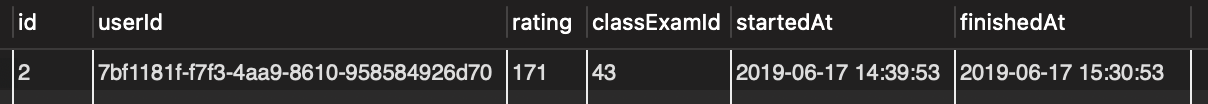
\includegraphics[width=8cm]{PrimerTabeleUser}
    \label{fig:example}%
\end{figure}

\begin{lstlisting}[language=SQL]
SELECT u.id, u.userId, u.rating, u.classExamId, a.startedAt, a.finishedAt 
FROM computed_user_ratings u JOIN exam_attempts a ON u.classExamId = a.classExamId 
WHERE u.classExamId=43;
\end{lstlisting}

\begin{figure}[h!]
    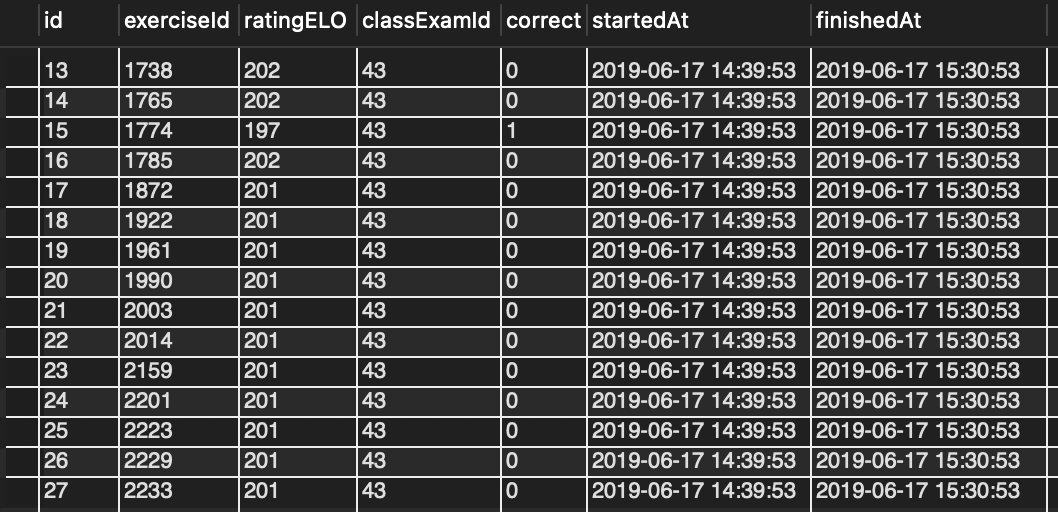
\includegraphics[width=8cm]{PrimerTabele}
    %\caption{Zapisi izračunov ratingov za izpit z identifikatorjem 43}%TODO: figure counting
    \label{fig:example}%
\end{figure}
\begin{lstlisting}[language=SQL]
SELECT e.id, e.exerciseId, e.ratingELO, e.classExamId, e.correct, a.startedAt, a.finishedAt 
FROM computed_exercise_ratings e JOIN exam_attempts a ON e.classExamId = a.classExamId 
WHERE e.classExamId=43;
\end{lstlisting}


\subsection{Trenutni rating sistem - ELO}
Pri oddaji kviza so pridobljeni prejšnji rating posameznih nalog v kvizu in prejšnji rating uporabnika. Za naloge in uporabnika so potem zaporedoma po nalogah izračunani novi ratingi po naslednjih enačbah:
\begin{equation}
    R'_{A}=R_{A}+K\cdot \left ( S_{A}-E_{A} \right )
\end{equation}
\begin{equation}
    E_{A}=\frac{Q_{A}}{Q_{A}+Q_{B}}
\end{equation}
Kjer so
\begin{equation}
    Q_{A}=10^{R_{A}/66}\;\;\;Q_{B}=10^{R_{B}/66}
\end{equation}
$S_{A}$ predstavlja dejanski izid, v primeru eQuiza 0 ali 1, $E_{A}$ pa pričakovan izid.
\hfill
\\
\\
$K$ je po navadi izračunan glede na število iger na katerih temelji trenuten rating (plus število iger v turnamentu pri šahu),
v trenutni implementaciji ratinga pa je privzet kot konstanten z vrednostjo 4,5
\hfill
\\
\\
Po takem postopku je bil po zgoraj opisanih algoritmih izračunan ELO rating na filtriranih podatkih z osnovnim ratingom 200.
%\newpage
%TODO normalne?
\begin{figure}[h!]
    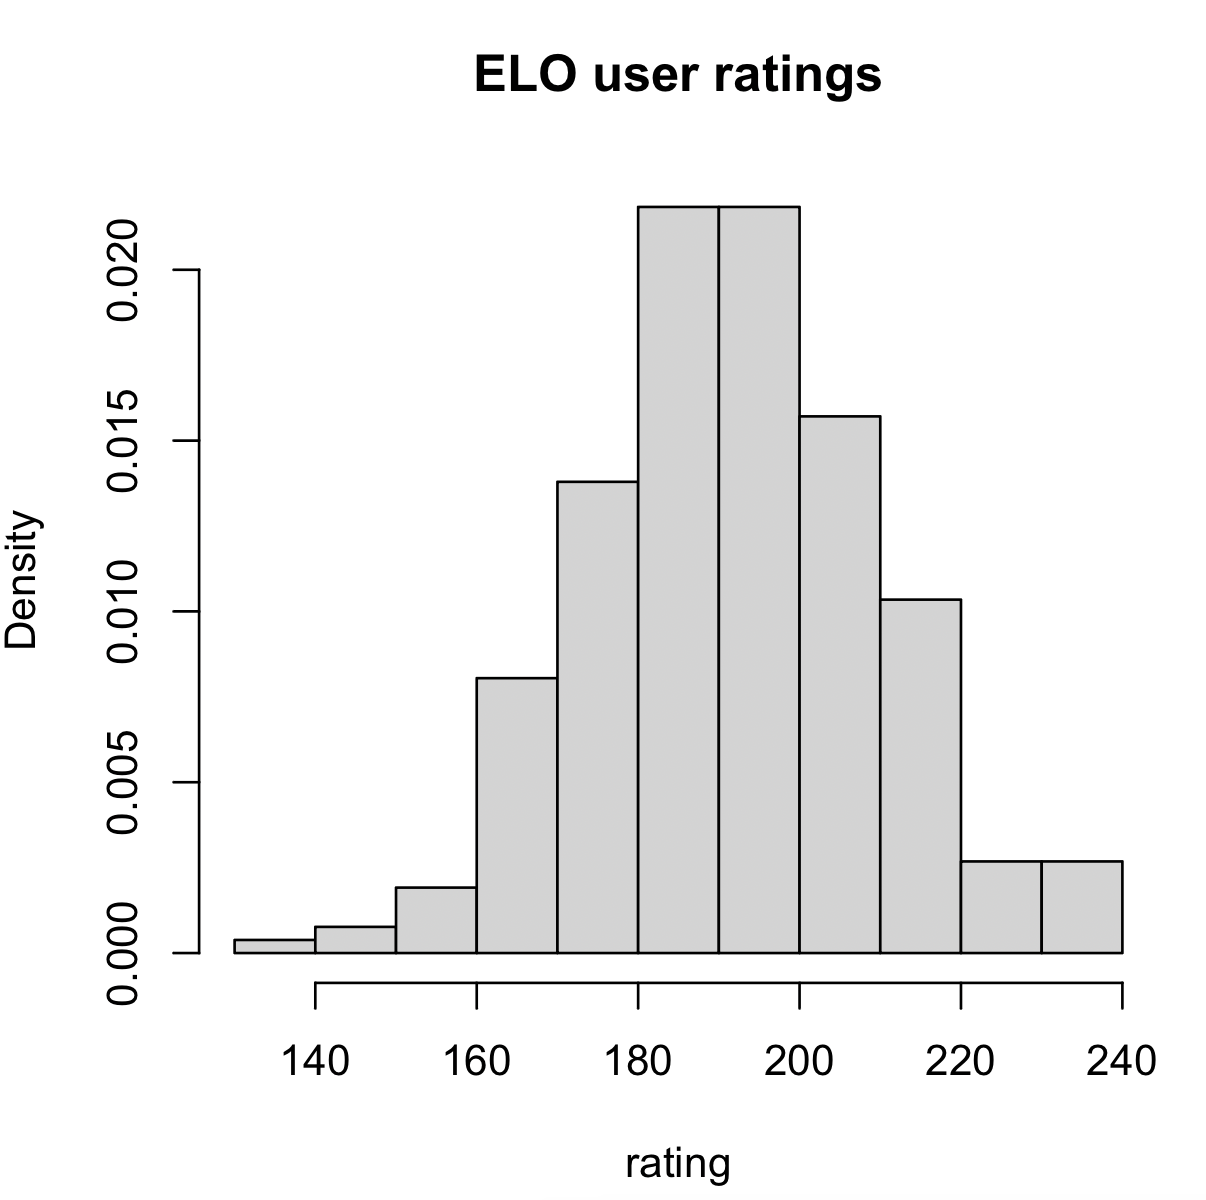
\includegraphics[width=8cm]{ComputedELO}
    \caption{Histogram končnih ELO ratingov uporabnikov}%TODO: figure counting
    \label{fig:example}%
\end{figure}
\begin{figure}[h!]
    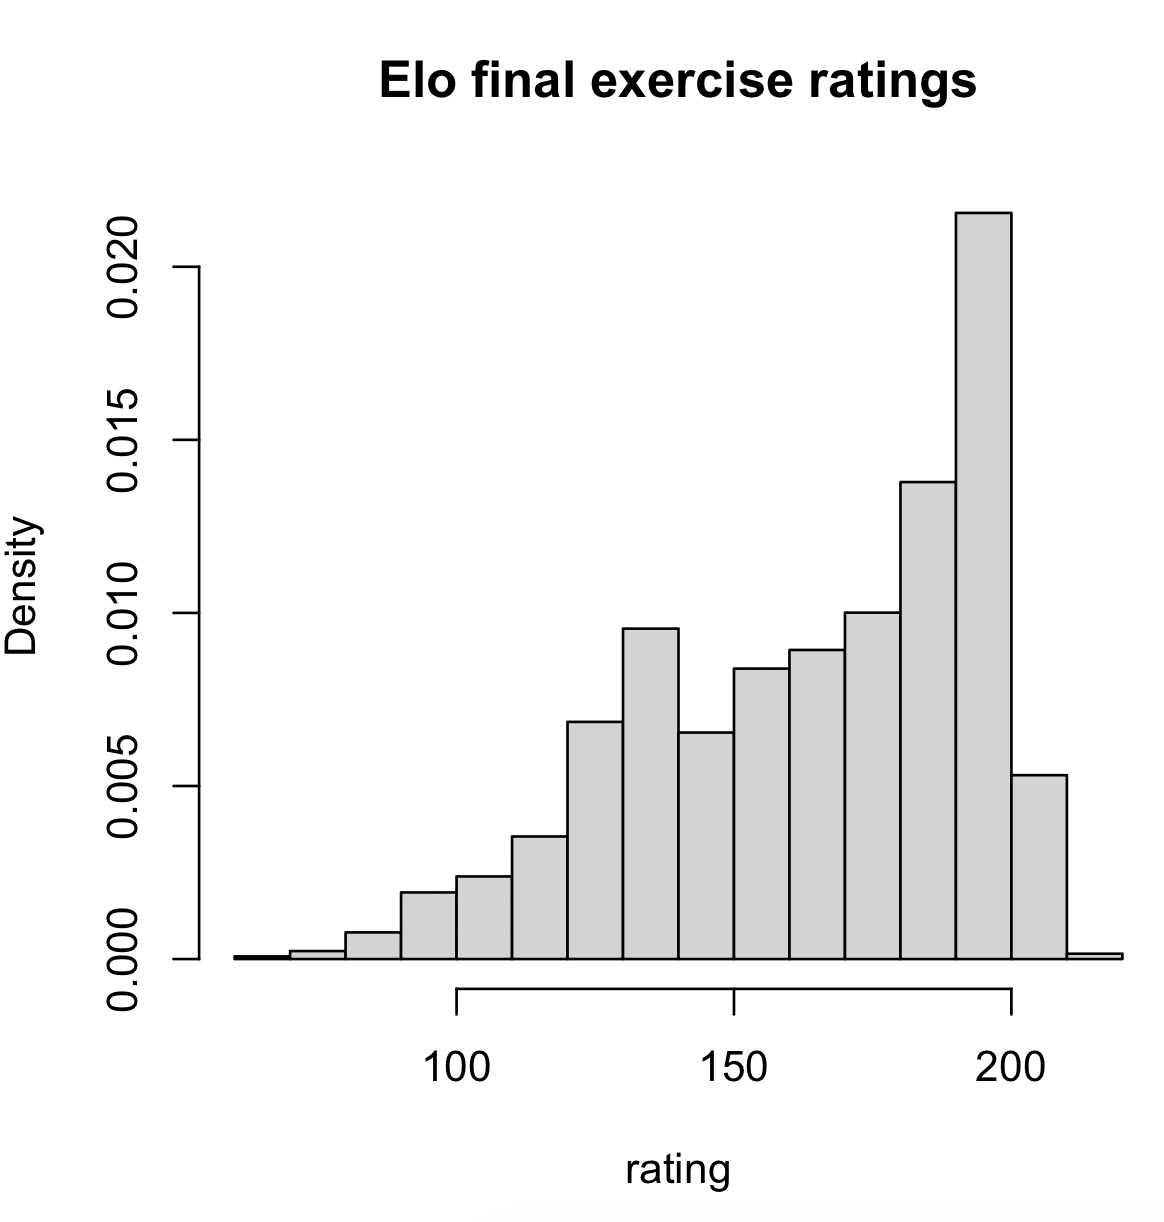
\includegraphics[width=8cm]{ComputedELOe}
    \caption{Histogram končnih ELO ratingov nalog}%TODO: figure counting
    \label{fig:example}%
\end{figure}
\hfill
\\
Zaradi velikega števila nalog iz katerih se naključno generira kviz, so posamezne naloge povprečno manjkrat ocenjene kot uprabniki, poleg tega pa so po številu rešenih kvizov med uporabniki velike razlike. 
\begin{figure}%
    \subfloat[\centering ]{{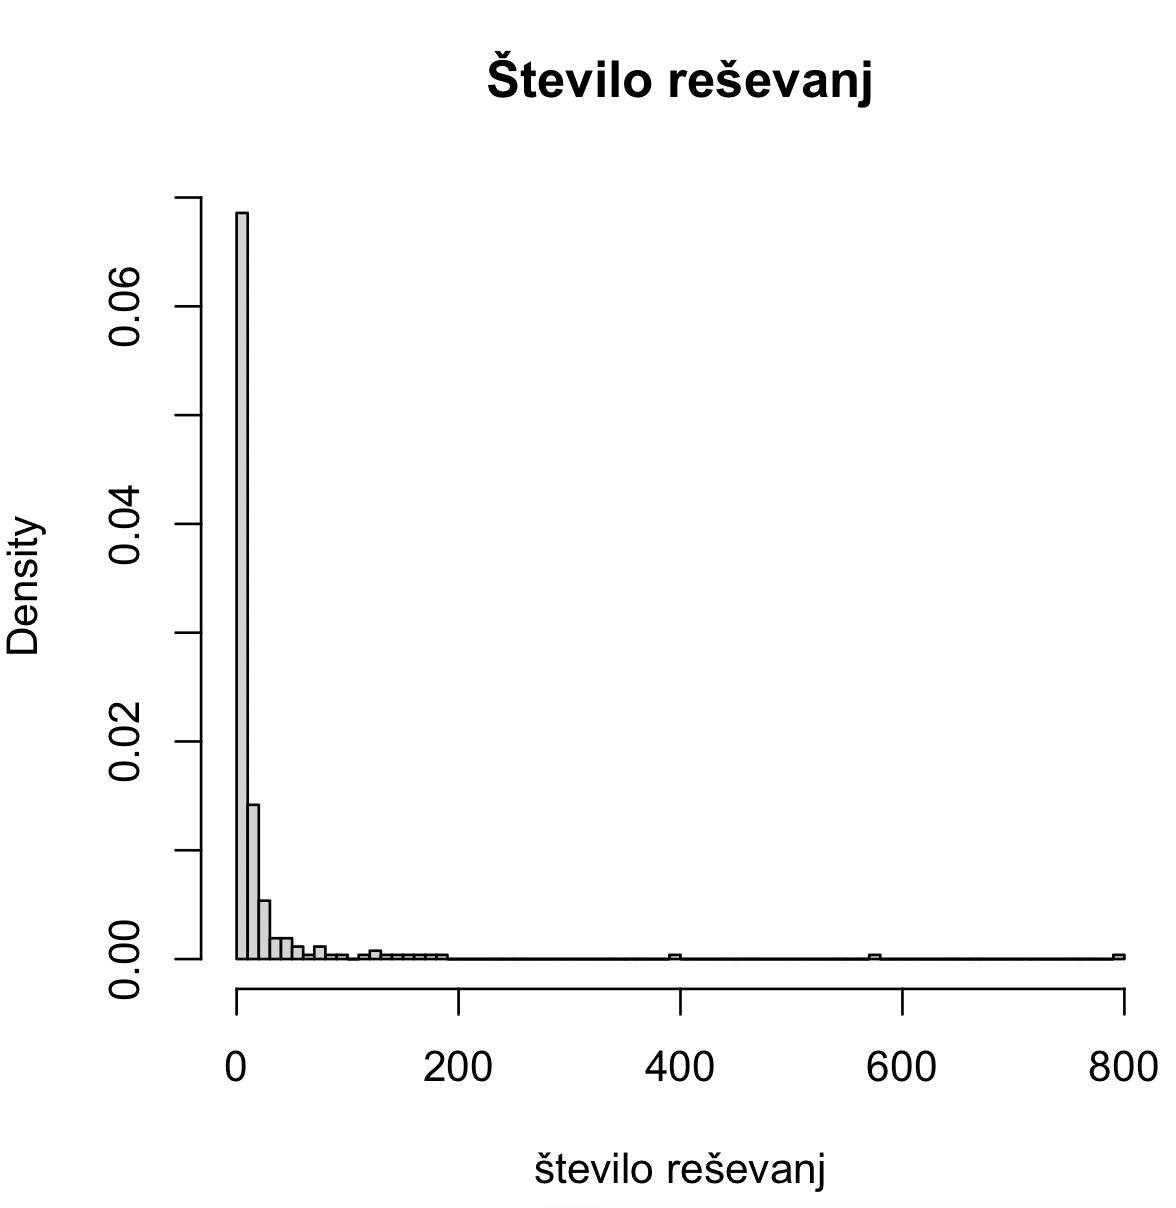
\includegraphics[width=4cm]{Resevanje} }}%
    \subfloat[\centering ]{{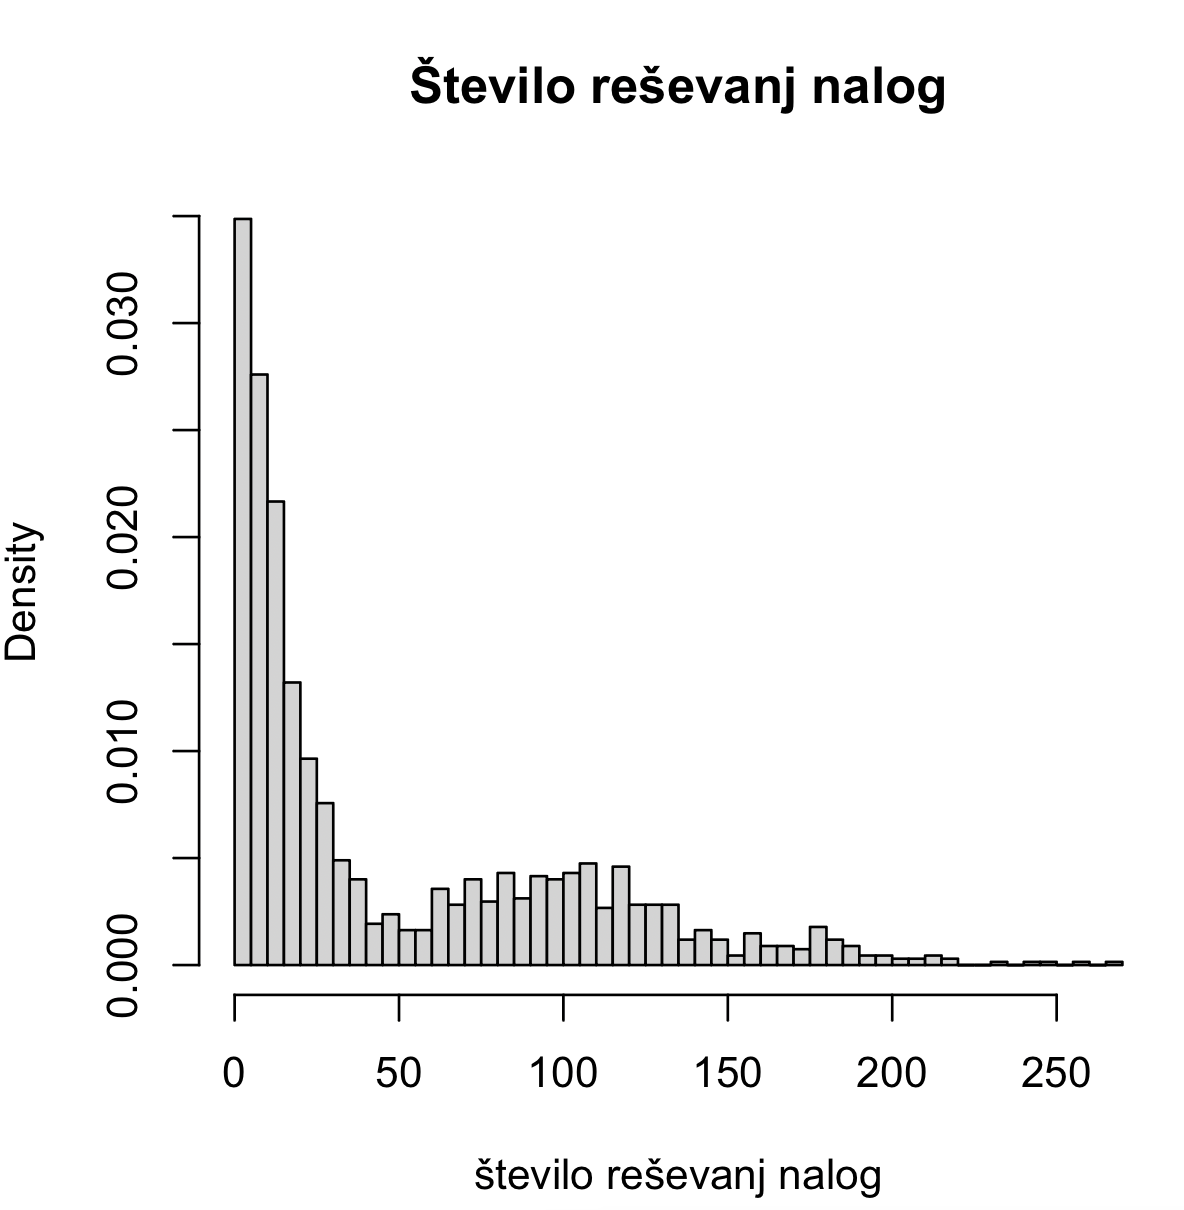
\includegraphics[width=4cm]{ResevanjeNalog} }}%
    \caption{Histogrami števila ratingov uporabnikov in nalog}%TODO: figure counting
    \label{fig:example}%
\end{figure}

Zaradi tega nekateri ratingi bazirajo na manj ali več ocenjevanjih in tako bolje ali slabše odražajo pravo sposobnost reševanja uporabnikov ali težavnost nalog. Zato je bil v nadaljevanju za enake podatke izračunan še Glicko rating.

\subsection{Glicko rating na pridobljenih podatkih}
%TODO: label?

Po enakem postopku kot ELO rating je bil zaporedno izračunan Glicko rating. Kot opisano v dokumentaciji Glicko ratinga, pa so bile naloge,
ki spadajo v isto iteracijo ocenjevanja obravnavane vsaka posebaj, kot več iger proti enako ocenjenem igralcu (uporabniku) in ne zaporedno z vmesnimi posodobitvami ratingov, kot v trenutnem rating sistemu.
\hfill
\\
\\
Za upoštevanje časov reševanj nalog, je potreben še izračun konstante $c$ kot parameter Glicko ratinga. Kot opisano v dokumentaciji lahko $c$
izračunamo glede na to, po kolikšnem času želimo, da $RD$ igralca pade na maksimalno vrednost, v tem primeru 350. Torej če v kontekstu ocenjevanj študentov privzamemo, da bo po preteklem času enega semestra, četudi ima študent na začetku minimalen $RD$ postal njegov rating nezanesljiv in pade njegov $RD$ na 350. Za tak čas je bilo vzetih 120dni.

\begin{equation}
    350=\sqrt{50^{2}+120\cdot c^{2}}
\end{equation}
\begin{equation}
    c\approx 32
\end{equation}

%TODO: beseda še o justificationu padanja ratinga skozi čas

\begin{figure}[h!]
    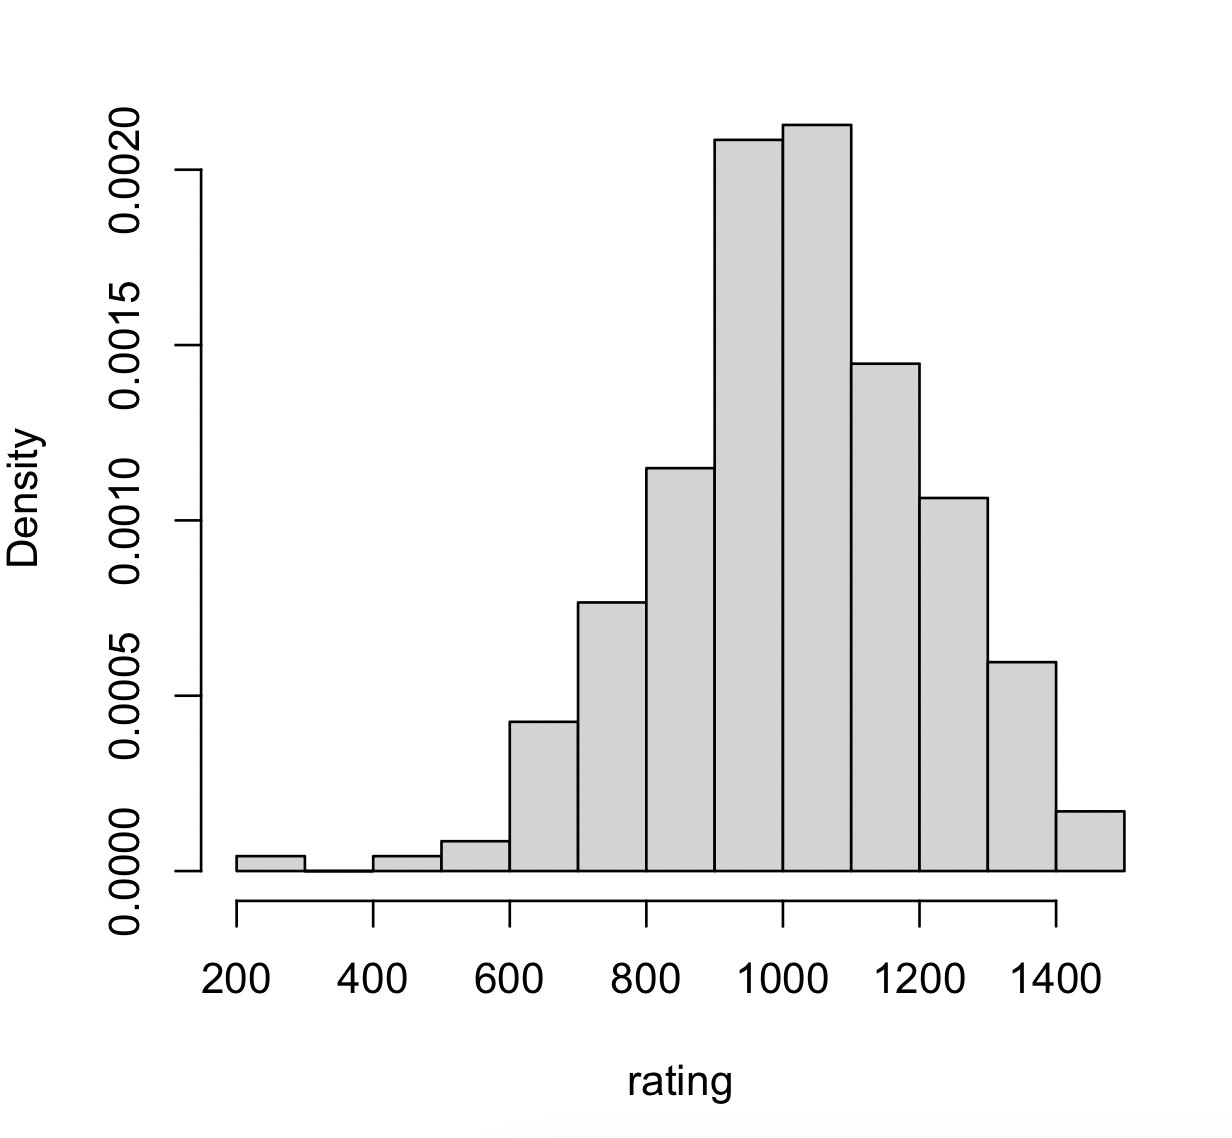
\includegraphics[width=8cm]{GlickoUser}
    \caption{Histogram končnih Glicko ratingov uporabnikov}%TODO: figure counting
    \label{fig:example}%
\end{figure}
\begin{figure}[h!]
    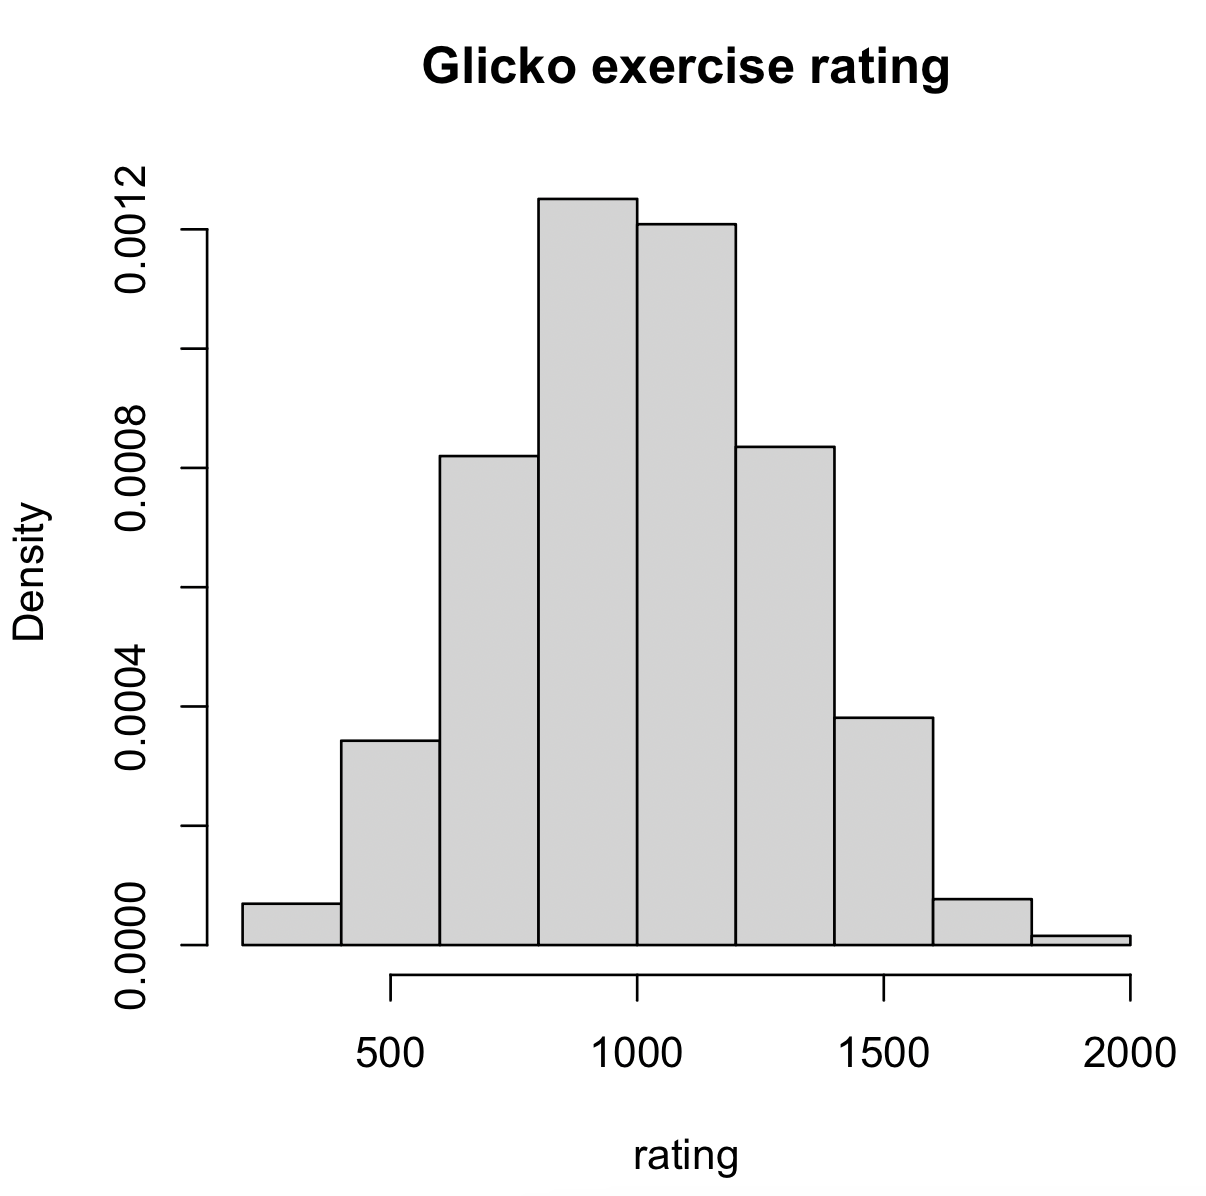
\includegraphics[width=8cm]{GlickoExercise}
    \caption{Histogram končnih Glicko ratingov nalog}%TODO: figure counting
    \label{fig:example}%
\end{figure}
\begin{figure}[h!]
    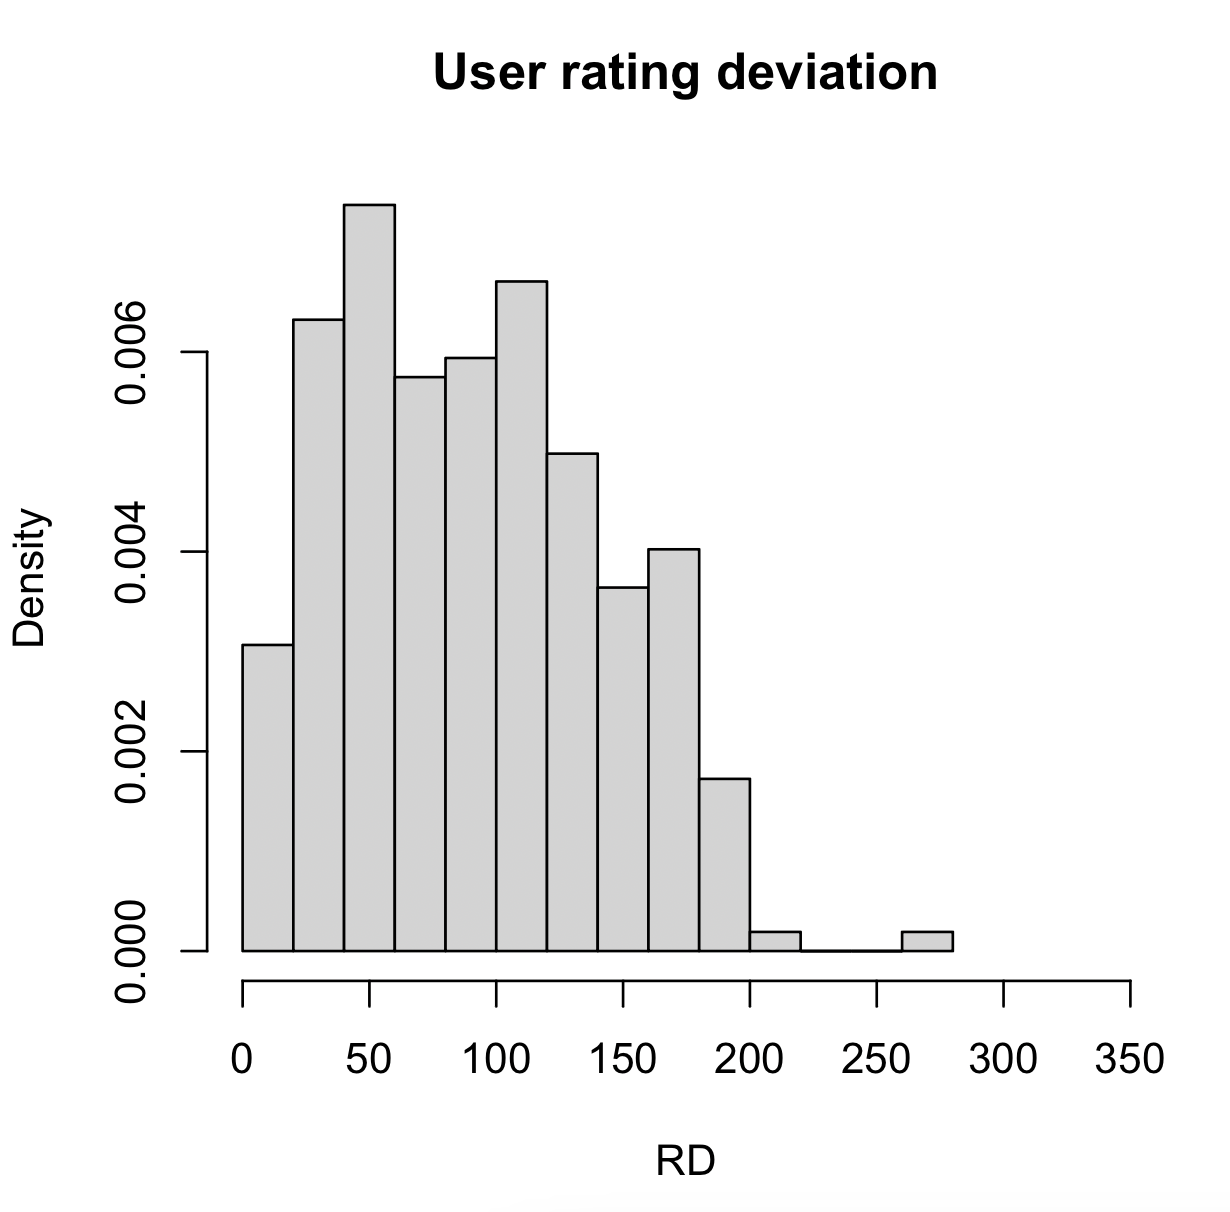
\includegraphics[width=8cm]{RDUser}
    \caption{Histogram končnih rating deviacij uporabnikov}%TODO: figure counting
    \label{fig:example}%
\end{figure}
\begin{figure}[h!]
    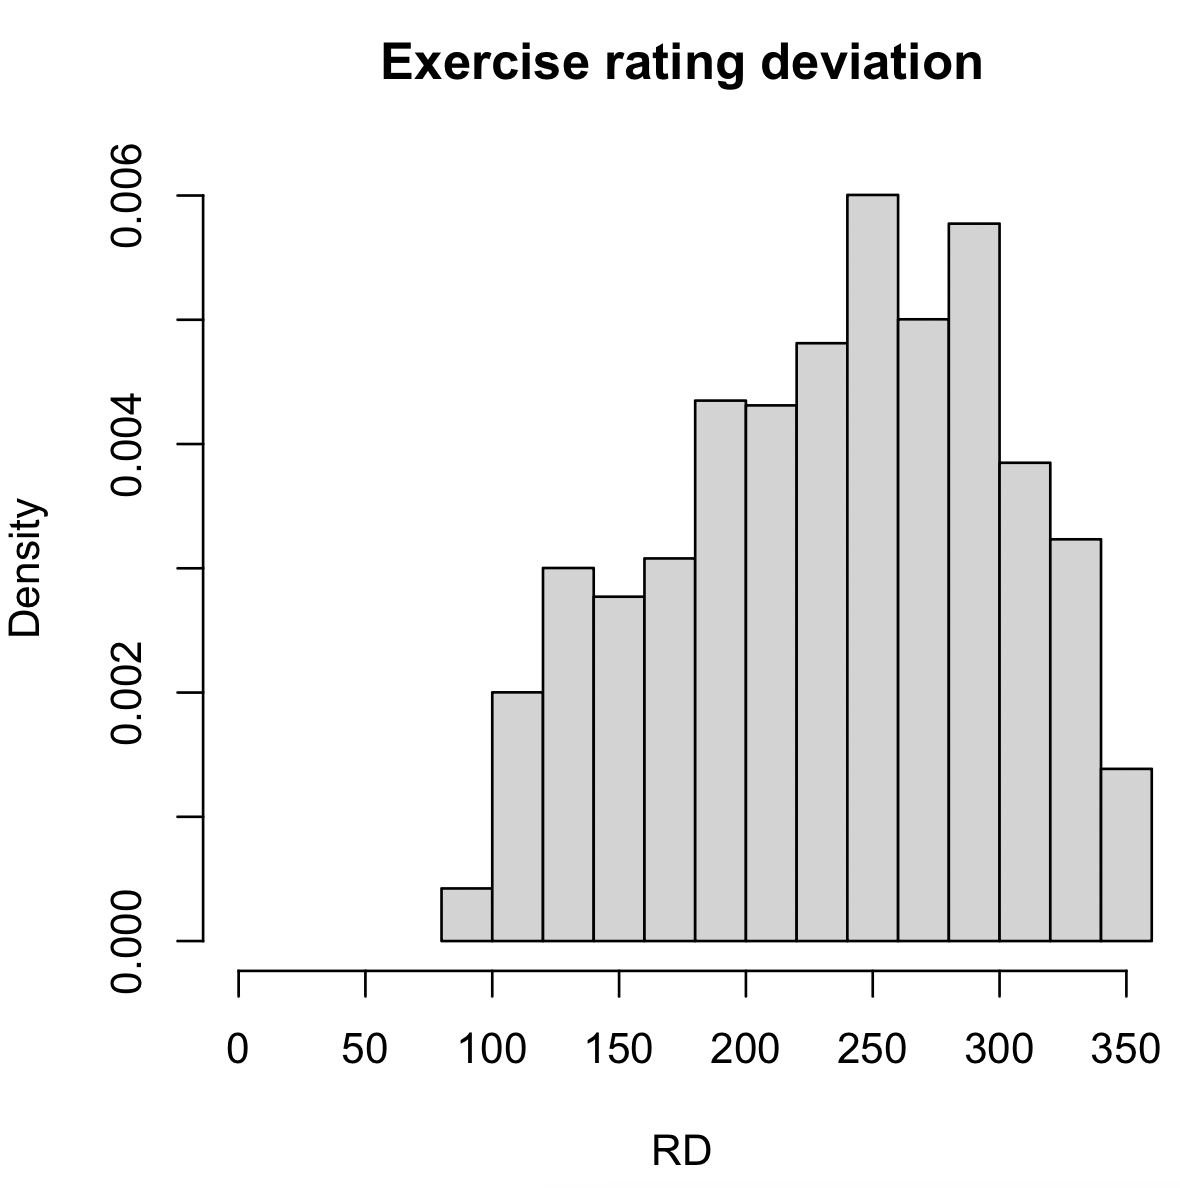
\includegraphics[width=8cm]{RDExercise}
    \caption{Histogram končnih rating deviacij nalog}%TODO: figure counting
    \label{fig:example}%
\end{figure}

\newpage
Opazimo, da je pri ratingu nalog $RD$ povprečno večji kot pri ratingu uporabnikov, saj so bile naloge povprečno manjkrat ocenjene ali pa bolj na redko (med ocenjevanji je preteklo več časa)
\hfill
\\

Ker smo za enoto vzeli dneve moramo za razlike v datumih ocenjevanj upoštevati razliko v dnevih, kjer naj bi se njegov $RD$ stalno spreminjal. Dovolj pa je, da $RD$ posodobimo samo pred novim ocenjevanjem ali pa ob vpogledu v rating študenta, da upoštevamo čas od njegovega zadnjega zabeleženega ocenjevanja. Za prikaz statistike glicko ratinga v tem primeru končni izračun deviacije ni bil izveden, saj so bila ocenjevanja izvedena v zelo različnih obdobjih od 2019 do 2023 in bi tako velik del študenov imel maksimalen $RD$. Za njihove ratinge to nima vpliva, saj se je med njihovimi ocenjevanji $RD$ prilagajal tudi po času. Tako lahko za posameznega študenta izračunamo tudi današnji $RD$ po formuli za $RD$ po preteklem času. %TODO link do formule 

\newpage

\begin{figure}[h!]
    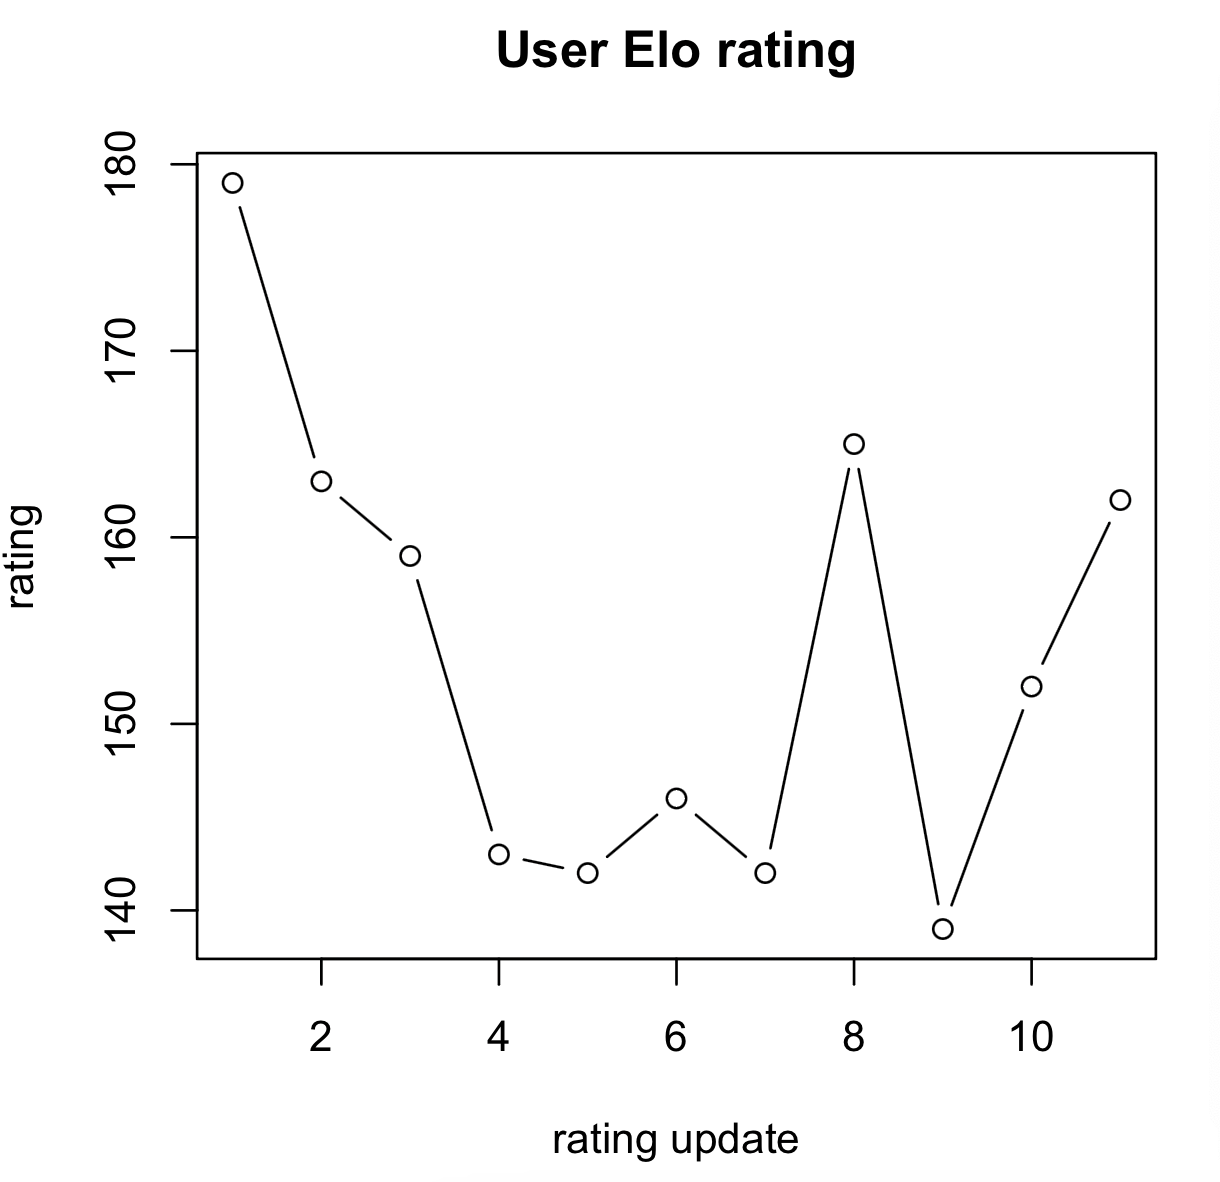
\includegraphics[width=8cm]{EloUserExample}
    \caption{Primer posodobitev ratinga za uporabnika pri ELO sistemu}%TODO: figure counting
    \label{fig:example}%
\end{figure}
\begin{figure}[h!]
    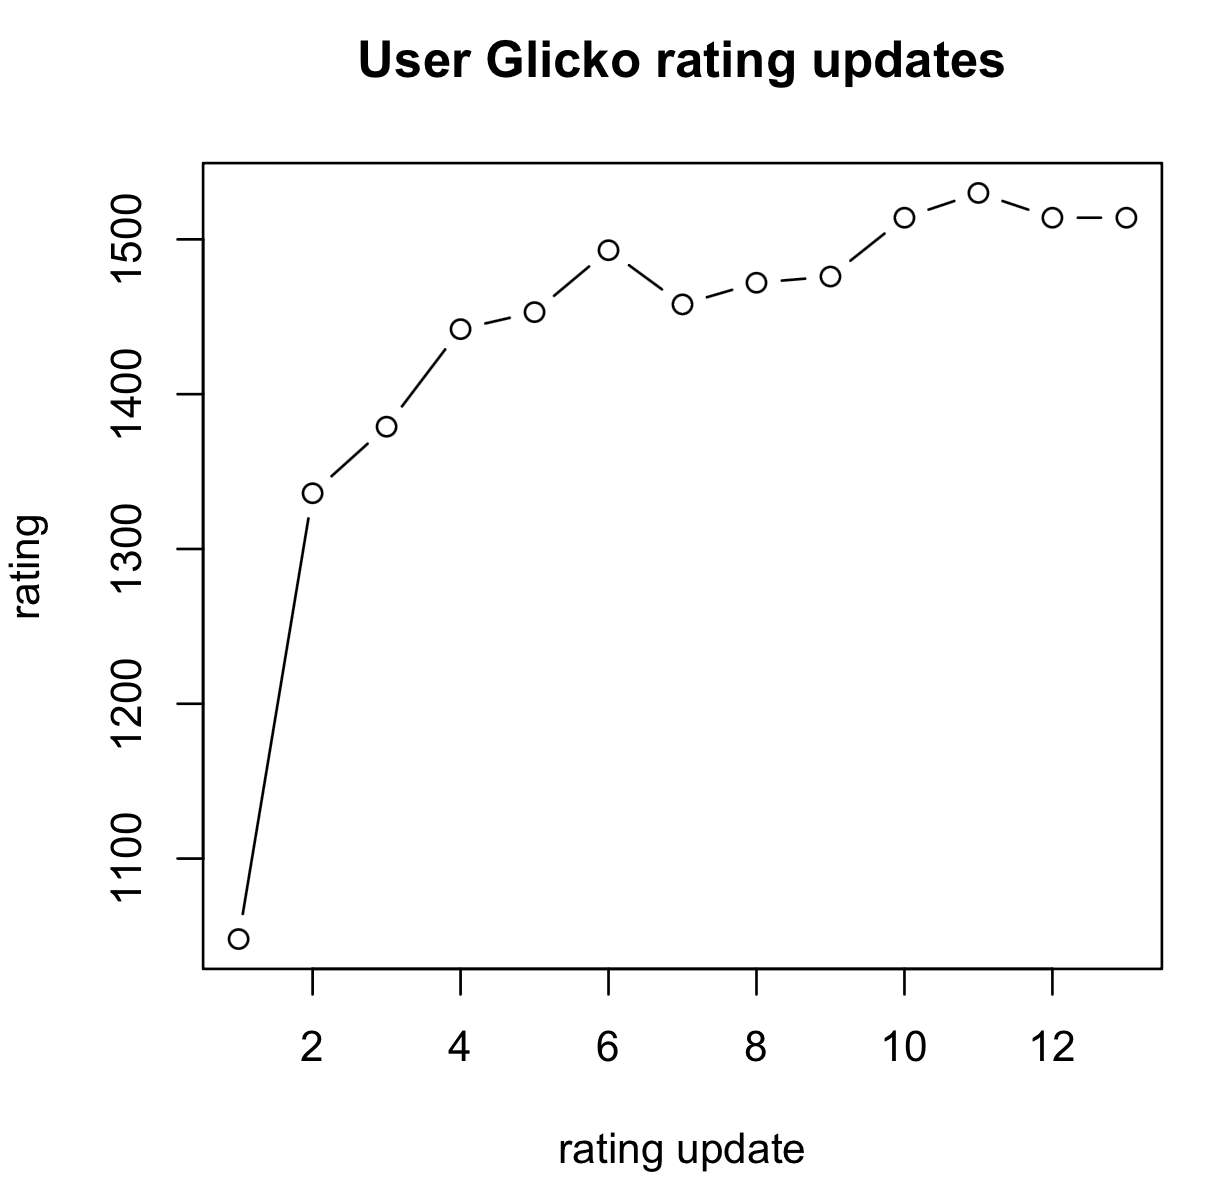
\includegraphics[width=8cm]{GlickoUserExample}
    \caption{Posodobitev ratinga za istega uporabnika pri Glicko sistemu}%TODO: figure counting
    \label{fig:example}%
\end{figure}

Za primer je bil vzet uporabnik, ki je vse ratinge pridobil v roku treh dni. , zato so spremembe v ratingu čedalje manjše, saj se njegov $RD$ hitro manjša.
\begin{figure}[h!]
    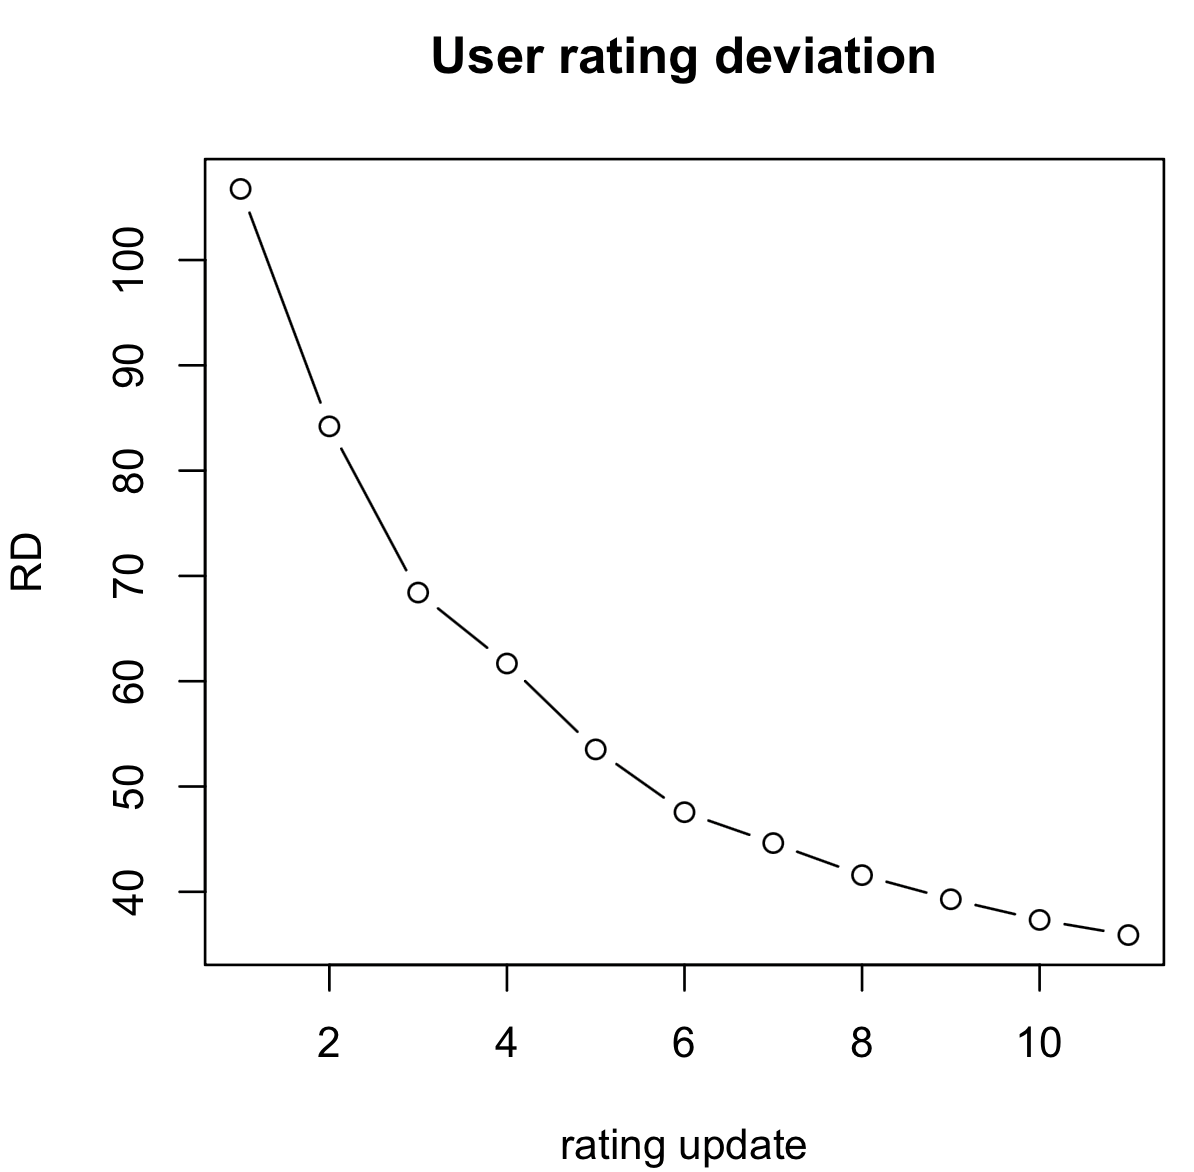
\includegraphics[width=8cm]{RDUserExample}
    \caption{Posodobitev RD za uporabnika}%TODO: figure counting
    \label{fig:example}%
\end{figure}
\newpage
Če vzamemo uporabnika z ratingi razporejenimi čez večji časovni interval, spremembe ratinga in $RD$ nista več nujno majhna. Skoke opazimo pri prvih ocenjevanjih po velikem časovnem intervalu brez posodobitev.

\begin{figure}[h!]
    \subfloat[\centering ]{{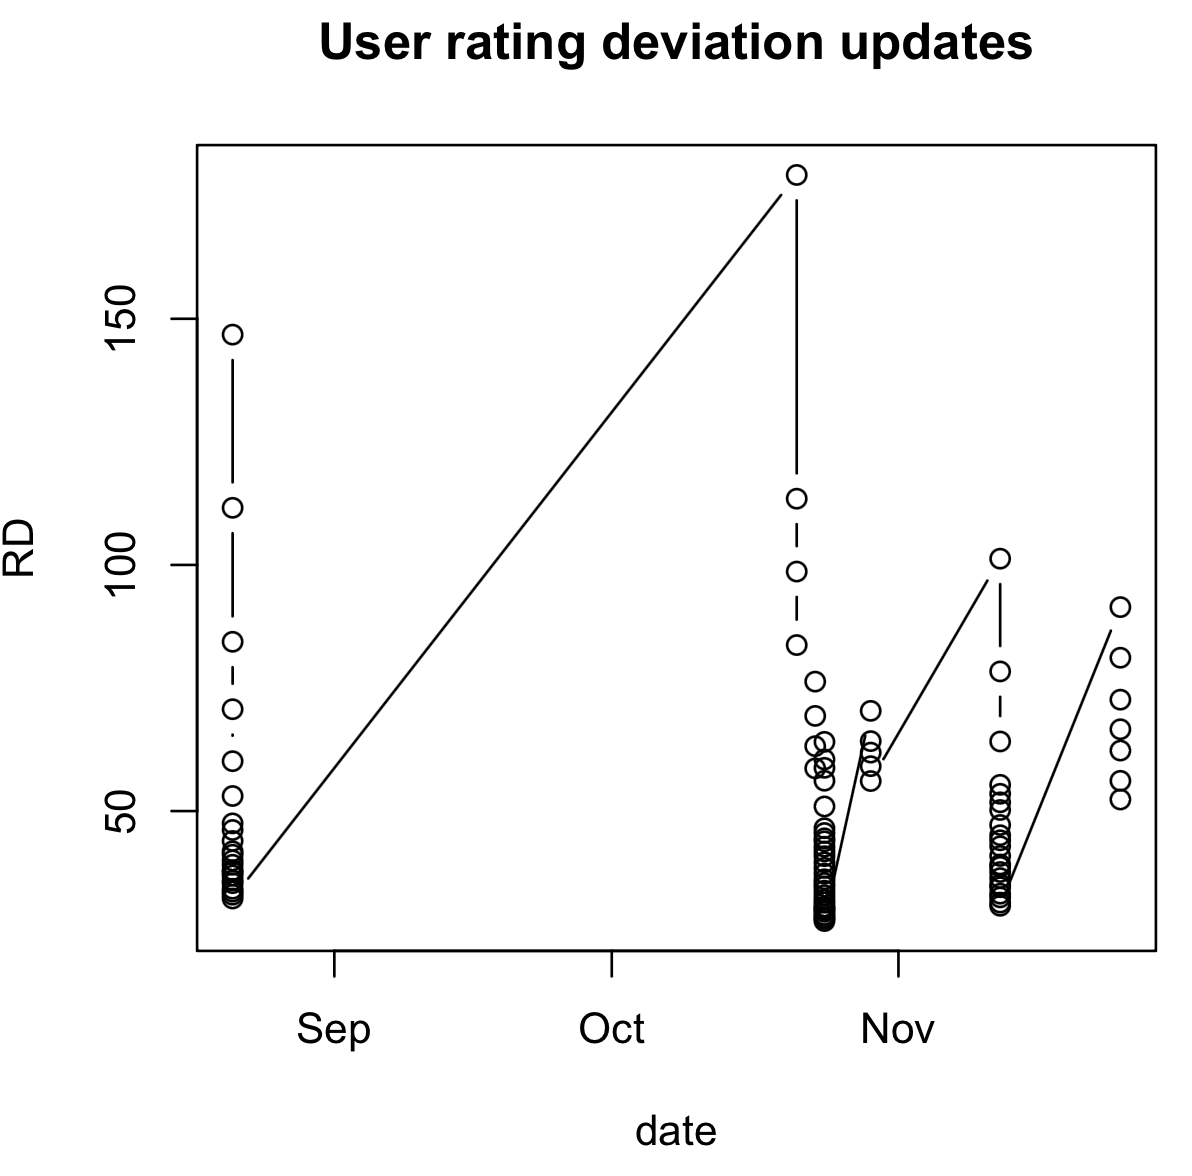
\includegraphics[width=4cm]{RDUserExampleBig} }}%
    \subfloat[\centering ]{{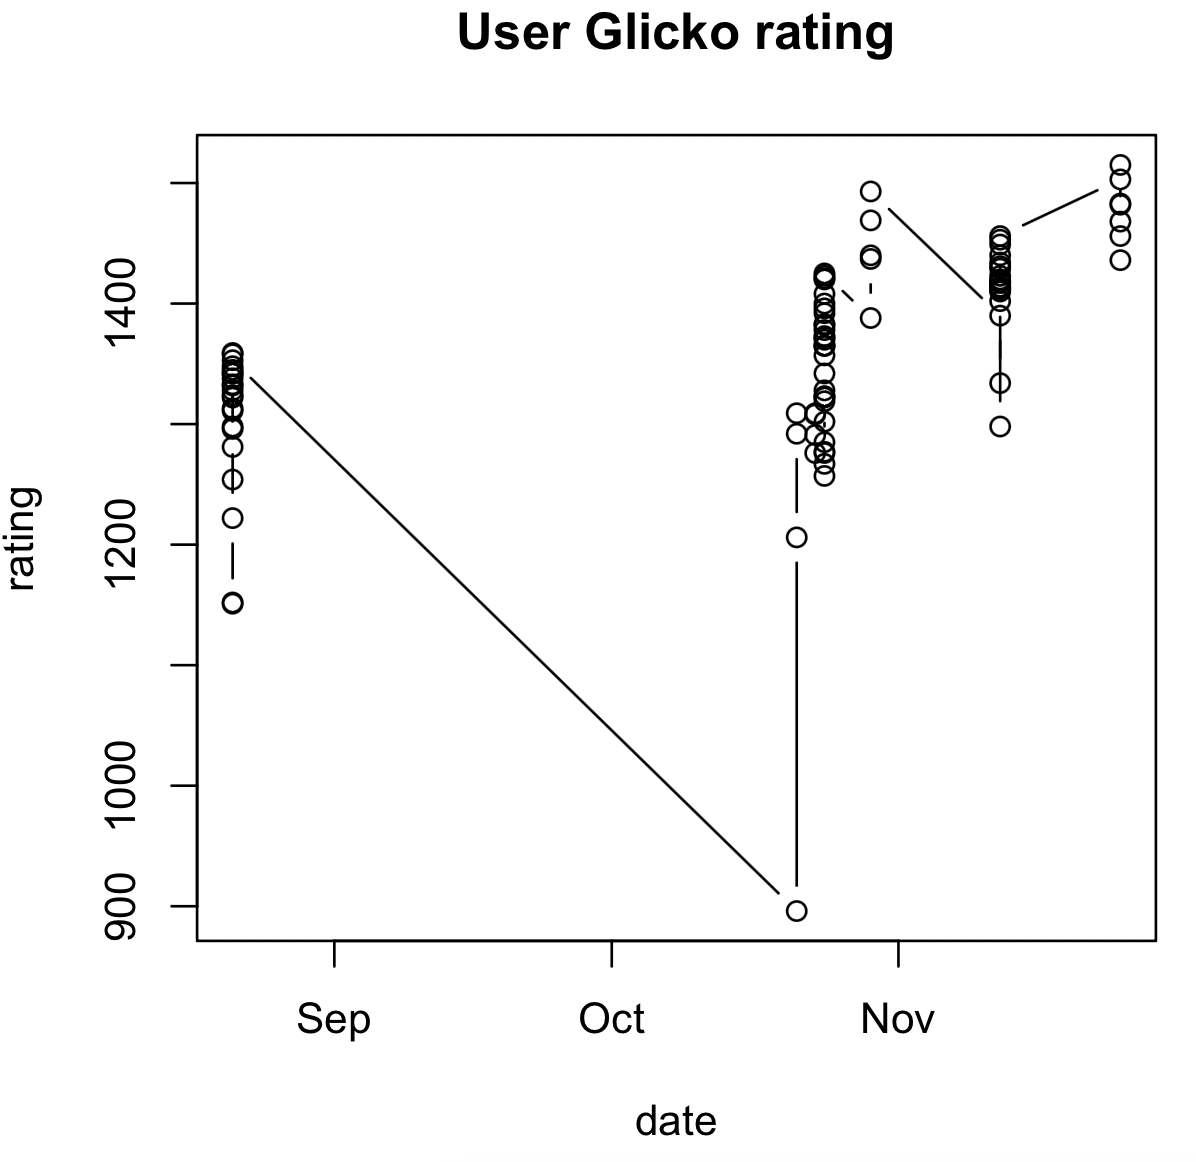
\includegraphics[width=4cm]{GlickoUserExampleBig} }}%
    \caption{Histogrami za Glicko pri uporabniku z več posodobitvami}%TODO: figure counting
    \label{fig:example}%
\end{figure}


\iffalse
Če študent reševal skozi semester izgleda rating po Elo tako: 

(Če pa nimamo rednih podatkov):
zgenerirana tabela resevanja po kolokvijih, sprothin kvizih in random resevanjih. Na random ratingih nalog zajetih iz equiz ali
pa ce je kaj informacije o tem.

iz zgornjih tabel se da ugotavljati kasnejse ugotovitve napisane spodaj

(morda) imamo informacijo samo o izpitu.
(primerjava ratinga Elo vs Glicko na izpitu, tudi za naloge)

Če 
Trenutni podaki (lahko) baza za nove,

Po rating updatih lahko dolocimo cas (in verjetno kaj je ucenec reseval) -- match lahko uporabimo kar prvi rating in matchamo casovno naslednje preizkuse

Ali imamo podatke nakljucnih resevanj? (Nejc Subic diplomska: Da?)
Ce ne lahko tudi umetno prikazemo ucinek za sprotno delo -- nakljucno izberem nekaj nalog(lahko tudi randomly generiram podobne podatke kot trenutne naloge v equizu).

\begin{itemize}
    \item Prikaz ratingov po izpitu (tudi za naloge). kot poseben primer za prikaz da je se vedno accurate -- izstopanje nalog
    \item Prikaz ratingov po rednih preverjanjih, kot prikaz kako se vzdrzuje rating in devianca(graf deviance za studenta) -- c samo pokaze koliko globoko bo dipnilo med preverjanji in s tem koliko pomembno je sprotno delo?
\end{itemize}

Zeljeni podatki:
\begin{itemize}
    \item izpit (sasa)
    \item cas posodobitev ratingov + kaj je ucenec takrat reseval (za sestavljene naloge (izpite) + nakljucno resevanje)
\end{itemize}
\hfill
\\
\\

\hfill
\\
\\
\begin{lemma} \label{lem:eps}
$\ell = \varepsilon + t(p-1)(q-1)$.
\end{lemma}

\begin{proof}
\begin{align*}
\ell &= \varepsilon + \B{r}(q-1) \\
&= \varepsilon + t(p-1)(q-1)
\end{align*}
\end{proof}

\begin{theorem} \label{thm:equiv}
$\ell \equiv \varepsilon \pmod{\varphi(n)}$.
\end{theorem}

\begin{proof}
By Lemma~\ref{lem:eps} and \eqref{eqn:phi} we have $\varepsilon \bmod{\varphi(n)} = \ell$.
\end{proof}

\begin{corollary} \label{cor:mult}
$\exists k \in \Z: \ell - \varepsilon = k \varphi(n)$.
\end{corollary}

\begin{proof}
Follows by Theorem~\ref{thm:equiv}.
\end{proof}
\fi

\section{Glicko za spremljanje študentov}
Z vpeljavo $RD$ pridobimo v primeru študentov informacijo o sprotnem delu, saj bo RD manjši za učence, ki so pogosteje ocenjeni. Če bi k ratingu pripomogli tudi, na primer redni kolokviji, bi reševanje dodatnih  naključnih reševanj kvizov/nalog bilo razvidno iz manjšega $RD$, kar kaže na več sprotnega dela in obratno. Za primer, pri predmetu Verjetnost in statistika se da predmet opraviti v celoti s sprotnimi preverjanji, kjer je snov enakomerno razdeljena na 5 kolokvijev skozi celoten semester. Torej bo študent, ki opravi samo eno preverjanje od petih ustrezno imel veliko deviacijo, saj imamo informacijo o njegovem znanju čedalje bolj nezanesljivo, ker vemo čedalje manj, koliko študent dejansko ve o Statistiki odkar je reševal tisti kolokvij.

Za nasprotnika učencu – nalogo, pa deviacija predstavlja kdaj je bila naloga nazadnje ocenjena, torej koliko je njena ocena zanesljiva. V primeru učenca, ki izbira naloge iz zbirke na equizu, bi lahko naloge z veliko deviacijo identificirali kot nepriljubljene (malo učencev se je lotilo naloge).

%TODO primer izpita?
%TODO tudi expected outcome

\hfill
\\
\\
V kontekstu igrifikacije eQuiza, lahko ratinge, predvsem pa $RD$ preslikamo v razrede iz katerih lahko bolj prijazno uporabniku spremljamo njegovo aktivnost na eQuizu. Iz statistike končnih $RD$ uporabnikov lahko uporabimo kvartile in razdelimo ratinge na 4 dele:

\begin{figure}[h!]
    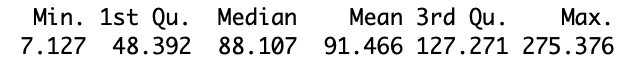
\includegraphics[width=8cm]{RDstat}
    \label{fig:example}%
\end{figure}

Tako lahko razporedimo uporabnike glede na njihove $RD$:
\hfill
\\
\\
$RD\leq48,392:\;visoka\;aktivnost$
\hfill
\\
$48,392<RD\leq88,107:\;srednje\;visoka\;aktivnost$
\hfill
\\
$88,107<RD\leq127.271:\;srednje\;nizka\;aktivnost$
\hfill
\\
$127.271<RD:\;nizka\;aktivnost$
\hfill




\lstset{basicstyle=\tiny,style=SQLstyle}
\begin{lstlisting}
\end{lstlisting}


%TODO: link do programov

\newpage
\section{Zakjuček}
\label{sec:cnc}

Glicko rating nam doda novo informacijo glede vloženega dela uporabnika. Dobimo informacijo o količini reševanj v določenem časovnem intervalu, posledično pa tudi zanesljivost ratinga izračunanega z Glicko, kjer je zanesljivost upoštevana tudi med samim računanjem. Poleg sprotnega dela pa dobimo informacijo tudi o reševanju nalog, njihovi težavnosti in priljubljenosti. Ker pri tem poskušamo zanseljivost zvečati, lahko z vpeljavo parametriziranih nalog
,ki jih tako večkrat uporabimo na preverjanjih, zvišamo zanesljivost njihovih ratingov. Če v rating vključimo še podatke iz izpitov in skupnih preverjanj, pa bo posledično rating še zanesljivejši, saj bo v isti iteraciji nalogo reševalo veliko učencev.

\hfill
\\
Kot je do sedaj algoritem operiral na trenutni podatkovni bazi eQuiza, lahko podoben algoritem uporabimo v nadaljevanju za beleženje ratingov na enak način, kot do sedaj. Implementacija Glicko ratinga za eQuiz je na voljo skupaj z vsemi programi uporabljenimi pri navedenih izračunih na GitHubu %TODO: link
\hfill
\\
\\
Za Glicko rating pa obstaja tudi bolj kompleksna izboljšana različica Glicko-2, ki bi lahko bila bolj primerna za dejansko implementacijo v aplikaciji %TODO: link

\bibliographystyle{babplain}
\bibliography{cite}

\end{document}
